\chapter{Arquitectura y tecnologías}
\label{chap:arquitectura}

Este capítulo presenta la arquitectura del sistema, las tecnologías utilizadas en cada componente con su justificación frente a las alternativas evaluadas, la arquitectura de despliegue, diferenciando lo diseñado de lo efectivamente desplegado, y los protocolos de comunicación entre componentes.

\section{Arquitectura lógica}
\label{sec:arquitectura-logica}
La arquitectura sigue la separación entre el punto de decisión de políticas (PDP) y el punto de aplicación de políticas (PEP) propuesta por NIST SP~800-207 \parencite{Rose2020}. El agente local actúa como PEP: observa la actividad, la informa y aplica la decisión, pero no evalúa el riesgo. La API central actúa como PDP: concentra el modelo, la política vigente y el estado de cada usuario, y decide la acción. Esta separación permite cambiar el modelo o la política sin modificar los agentes instalados.

El sistema no es una aplicación monolítica sino un conjunto de componentes con funciones y entornos de ejecución distintos, organizados en un único repositorio con cinco subsistemas: la API de \emph{scoring}, el agente, el \emph{dashboard}, el \emph{pipeline} de entrenamiento y los \emph{scripts} de demostración, ensayo y validación. La API es el único punto de acceso al estado y a la configuración, y la utilizan cuatro tipos de consumidores con distintos niveles de acceso:
\begin{itemize}
	\item \textbf{Agente:} envía eventos y confirma las acciones ejecutadas, con una clave propia que solo habilita esas dos operaciones.
	\item \textbf{\emph{Dashboard} en modo consulta:} lee el estado de los usuarios, el historial y la configuración.
	\item \textbf{\emph{Dashboard} en modo administración:} además, modifica la configuración y reinicia usuarios.
	\item \textbf{Público:} solo accede a la salud del servicio y al inicio de sesión.
\end{itemize}

El flujo principal comienza en el agente, que captura un evento y lo envía a la API. La API lo valida, actualiza el estado del usuario en Redis, persiste el evento crudo en PostgreSQL, calcula el puntaje y responde con el nivel y la acción. El agente ejecuta la acción y confirma el resultado. En paralelo, el \emph{dashboard} consulta periódicamente la API para mostrar el estado actualizado, y el planificador de la API dispara el reentrenamiento cuando corresponde.

\section{Lenguajes de programación}
\label{sec:lenguajes}
Cada componente utiliza el lenguaje que mejor se ajusta a su función y a su entorno de ejecución. La tabla~\ref{tab:lenguajes} resume la elección.

\begin{longtable}{>{\raggedright\arraybackslash}p{2.4cm}>{\raggedright\arraybackslash}p{3.6cm}>{\raggedright\arraybackslash}p{8.1cm}}
	\caption{Lenguajes de programación utilizados}
	\label{tab:lenguajes}\\
	\hline
	\textbf{Lenguaje} & \textbf{Dónde se usa} & \textbf{Justificación} \\
	\hline
	\endfirsthead
	\hline
	\textbf{Lenguaje} & \textbf{Dónde se usa} & \textbf{Justificación} \\
	\hline
	\endhead
	Python & API, agente, \emph{pipeline} de entrenamiento y \emph{scripts} & Es el lenguaje del ecosistema de aprendizaje automático utilizado (scikit-learn y TensorFlow). Usarlo también en la API permite reutilizar el código de cálculo del puntaje validado durante el entrenamiento, sin reimplementarlo en otro lenguaje, y reduce el riesgo de diferencias entre lo validado y lo que se ejecuta en producción. El desarrollo utiliza Python~3.12; la integración continua y el servidor, Python~3.11. \\
	\hline
	TypeScript & \emph{Dashboard} & El \emph{dashboard} modifica configuraciones que cambian el comportamiento del agente, como los umbrales y la acción por nivel. El tipado estático detecta errores de estructura durante el desarrollo, y la validación con Zod los detecta en tiempo de ejecución sobre los datos recibidos de la API. \\
	\hline
	PowerShell & Instalación del agente y despliegue & Es la herramienta de automatización nativa de Windows. Se utiliza para registrar el arranque automático del agente y para publicar versiones de la API en la nube desde el equipo de desarrollo. \\
	\hline
	HCL (Terraform) y Bash & Infraestructura en la nube & HCL describe la infraestructura como código; Bash configura el servidor en su primer arranque. \\
	\hline
\end{longtable}

Se descartó un \emph{backend} en Node.js porque igualmente habría requerido un servicio en Python para los modelos, y Java con Spring Boot porque implicaba más configuración y código para el alcance del proyecto.

\section{Frameworks y librerías}
\label{sec:frameworks}

Esta sección describe los \emph{frameworks} y las librerías de cada componente: la API de \emph{scoring}, el agente, el \emph{dashboard} y el \emph{pipeline} de entrenamiento. Para cada elección se indican las alternativas evaluadas.

\subsection{API de \emph{scoring}}
\begin{longtable}{>{\raggedright\arraybackslash}p{3.4cm}>{\raggedright\arraybackslash}p{10.7cm}}
	\caption{Frameworks y librerías de la API}
	\label{tab:tec-api}\\
	\hline
	\textbf{Tecnología} & \textbf{Justificación} \\
	\hline
	\endfirsthead
	\hline
	\textbf{Tecnología} & \textbf{Justificación} \\
	\hline
	\endhead
	FastAPI 0.104 y Uvicorn & Soporte asincrónico, validación automática de la entrada y la salida, y documentación OpenAPI generada a partir del código, útil para una API de 31 \emph{endpoints}. Flask habría requerido extensiones para llegar al mismo resultado. \\
	\hline
	Pydantic 2 & Define los contratos de datos que comparten el agente, la API y el \emph{dashboard}. Un evento mal formado se rechaza automáticamente, sin código de validación manual. \\
	\hline
	SQLAlchemy y psycopg2 & Acceso a PostgreSQL con consultas SQL explícitas y un grupo de conexiones reducido. Las escrituras son de dos tipos: una por evento en la tabla de eventos crudos y una por usuario y día en el historial. Los tiempos de espera acotados evitan que una caída de la base de datos bloquee la evaluación de eventos. \\
	\hline
	redis-py & Cliente de Redis para el estado de cada usuario, que se lee y escribe en cada evento. Se eligió Redis frente a PostgreSQL para este estado porque el patrón es de alta frecuencia y baja latencia, distinto del historial. Redis ofrece además transacciones optimistas, que la API utiliza con hasta 20 reintentos ante escrituras concurrentes. \\
	\hline
	scikit-learn 1.4 & Implementación madura de Isolation Forest. Se prefirió frente a autoencoders tabulares o máquinas de vectores de soporte de una clase por su bajo costo computacional y porque su salida se presta a la explicación por variables. \\
	\hline
	TensorFlow 2.16 (Keras) & Implementación del LSTM Autoencoder, que analiza el orden de los eventos, algo que Isolation Forest no captura al trabajar con agregados diarios. Se eligió Keras frente a PyTorch por su API de alto nivel. \\
	\hline
	pandas, NumPy, SciPy y joblib & Manipulación de datos, cálculo numérico y serialización de los modelos entrenados. Todas las dependencias de la API están fijadas en versiones exactas para que el cálculo sea reproducible. \\
	\hline
	requests & Consultas al proveedor IAM y a servicios externos. \\
	\hline
	pytest & Pruebas automatizadas de la API y del agente. \\
	\hline
\end{longtable}

\subsection{Agente}
\begin{longtable}{>{\raggedright\arraybackslash}p{3.4cm}>{\raggedright\arraybackslash}p{10.7cm}}
	\caption{Librerías del agente}
	\label{tab:tec-agente}\\
	\hline
	\textbf{Tecnología} & \textbf{Justificación} \\
	\hline
	\endfirsthead
	\hline
	\textbf{Tecnología} & \textbf{Justificación} \\
	\hline
	\endhead
	psutil & Enumeración de procesos y conexiones de red desde Python sin invocar directamente la API de Windows. \\
	\hline
	requests & Envío de eventos a la API. El agente envía en forma secuencial y no necesita un cliente asincrónico. \\
	\hline
	python-dotenv & Carga de la configuración local del agente, como la dirección de la API y su clave. \\
	\hline
	icacls (sistema operativo) & Herramienta nativa de Windows para modificar los permisos de carpetas en las mitigaciones de denegación y su reversión. \\
	\hline
\end{longtable}

El agente tiene solo tres dependencias externas. Como se ejecuta en segundo plano en el equipo del usuario, minimizar las dependencias reduce la superficie de ataque y el consumo de recursos.

\subsection{\emph{Dashboard}}
\begin{longtable}{>{\raggedright\arraybackslash}p{3.4cm}>{\raggedright\arraybackslash}p{10.7cm}}
	\caption{Frameworks y librerías del \emph{dashboard}}
	\label{tab:tec-frontend}\\
	\hline
	\textbf{Tecnología} & \textbf{Justificación} \\
	\hline
	\endfirsthead
	\hline
	\textbf{Tecnología} & \textbf{Justificación} \\
	\hline
	\endhead
	React 19 & Componentes reutilizables entre pantallas, como los indicadores de nivel, cobertura y aprendizaje. \\
	\hline
	Vite 8 & Arranque y recarga en caliente más rápidos que las herramientas basadas en Webpack. \\
	\hline
	TypeScript y Zod 4 & Doble validación de los datos: en compilación y en ejecución. \\
	\hline
	TanStack Query 5 & Caché, revalidación y consulta periódica cada 2 segundos sin escribir a mano la lógica de recarga, carga y error de cada consulta. Permite reflejar al instante un cambio de configuración recién guardado. \\
	\hline
	React Router 7 & Navegación entre las ocho pantallas, con rutas protegidas por el inicio de sesión. \\
	\hline
	Recharts 3 & Gráfico de la evolución del puntaje, integrado al modelo de componentes de React. \\
	\hline
	Tailwind CSS 4 & Estilos utilitarios y tema claro y oscuro sin hojas de estilo separadas. \\
	\hline
	Oxlint & Análisis estático rápido, integrado a la integración continua. \\
	\hline
\end{longtable}

\subsection{\emph{Pipeline} de entrenamiento}
\begin{longtable}{>{\raggedright\arraybackslash}p{3.4cm}>{\raggedright\arraybackslash}p{10.7cm}}
	\caption{Herramientas del \emph{pipeline} de entrenamiento}
	\label{tab:tec-pipeline}\\
	\hline
	\textbf{Tecnología} & \textbf{Justificación} \\
	\hline
	\endfirsthead
	\hline
	\textbf{Tecnología} & \textbf{Justificación} \\
	\hline
	\endhead
	Jupyter & Las seis fases del \emph{pipeline}, desde la exploración hasta el puntaje híbrido, son \emph{notebooks}: el trabajo de preparación y entrenamiento es exploratorio e iterativo, y los \emph{notebooks} conservan el código junto con sus resultados. \\
	\hline
	nbconvert & Ejecución de los \emph{notebooks} sin interfaz, en un proceso separado de la API, cuando el planificador dispara un reentrenamiento. \\
	\hline
	DuckDB & Consultas SQL sobre el archivo del conjunto de datos (14~GB en formato JSON por líneas) sin cargarlo en memoria ni administrar un motor de base de datos aparte. \\
	\hline
\end{longtable}

\section{Servicios e infraestructura}
\label{sec:servicios}
\begin{longtable}{>{\raggedright\arraybackslash}p{3.4cm}>{\raggedright\arraybackslash}p{10.7cm}}
	\caption{Servicios externos e infraestructura}
	\label{tab:servicios}\\
	\hline
	\textbf{Servicio} & \textbf{Uso y justificación} \\
	\hline
	\endfirsthead
	\hline
	\textbf{Servicio} & \textbf{Uso y justificación} \\
	\hline
	\endhead
	Redis gestionado (Upstash) & Estado operativo y configuración. Un servicio gestionado evita administrar una instancia propia y es accesible tanto desde el entorno local como desde la nube. \\
	\hline
	PostgreSQL gestionado (Supabase) & Historial, eventos crudos, auditoría y métricas. Incluye seguridad a nivel de fila y la extensión criptográfica que usa la cadena de \emph{hashes}. \\
	\hline
	Amazon Web Services & Infraestructura para el despliegue: instancia de cómputo para la API, almacenamiento de objetos para el \emph{dashboard} y las versiones publicadas, almacén de parámetros para los secretos y red de distribución de contenidos para publicar el \emph{dashboard} con HTTPS. \\
	\hline
	Terraform & Infraestructura como código: los recursos de la nube se crean, modifican y destruyen de forma reproducible y revisable. \\
	\hline
	GitHub Actions & Integración continua: análisis estático, compilación, pruebas y validación de la infraestructura en cada cambio. \\
	\hline
	Correo SMTP & Notificaciones al administrador. Es opcional: sin servidor configurado, la notificación solo se registra. \\
	\hline
	Gemini & Redacción asistida del correo de notificación. Es opcional y tiene un texto predefinido de respaldo, por lo que la notificación no depende de un servicio externo. \\
	\hline
	Keycloak & Proveedor IAM de referencia para el adaptador de identidad. Es opcional y está desactivado por defecto. \\
	\hline
\end{longtable}

\section{Arquitectura de despliegue}
\label{sec:despliegue}
El sistema tiene dos arquitecturas de despliegue: la local, verificada de extremo a extremo, y la de la nube, diseñada y aplicada en forma parcial.

\subsection{Despliegue local}
En el entorno local, el agente, la API y el \emph{dashboard} se ejecutan como procesos nativos en un equipo Windows y se conectan a Redis y PostgreSQL gestionados (figura~\ref{fig:despliegue-local}). El agente se comunica con la API por la interfaz de red local y el \emph{dashboard} la consulta desde el servidor de desarrollo. Opcionalmente, la API consulta un proveedor IAM simulado o Keycloak. Todas las pruebas funcionales y demostraciones se realizaron sobre esta configuración.

\begin{figure}[ht]
	\centering
	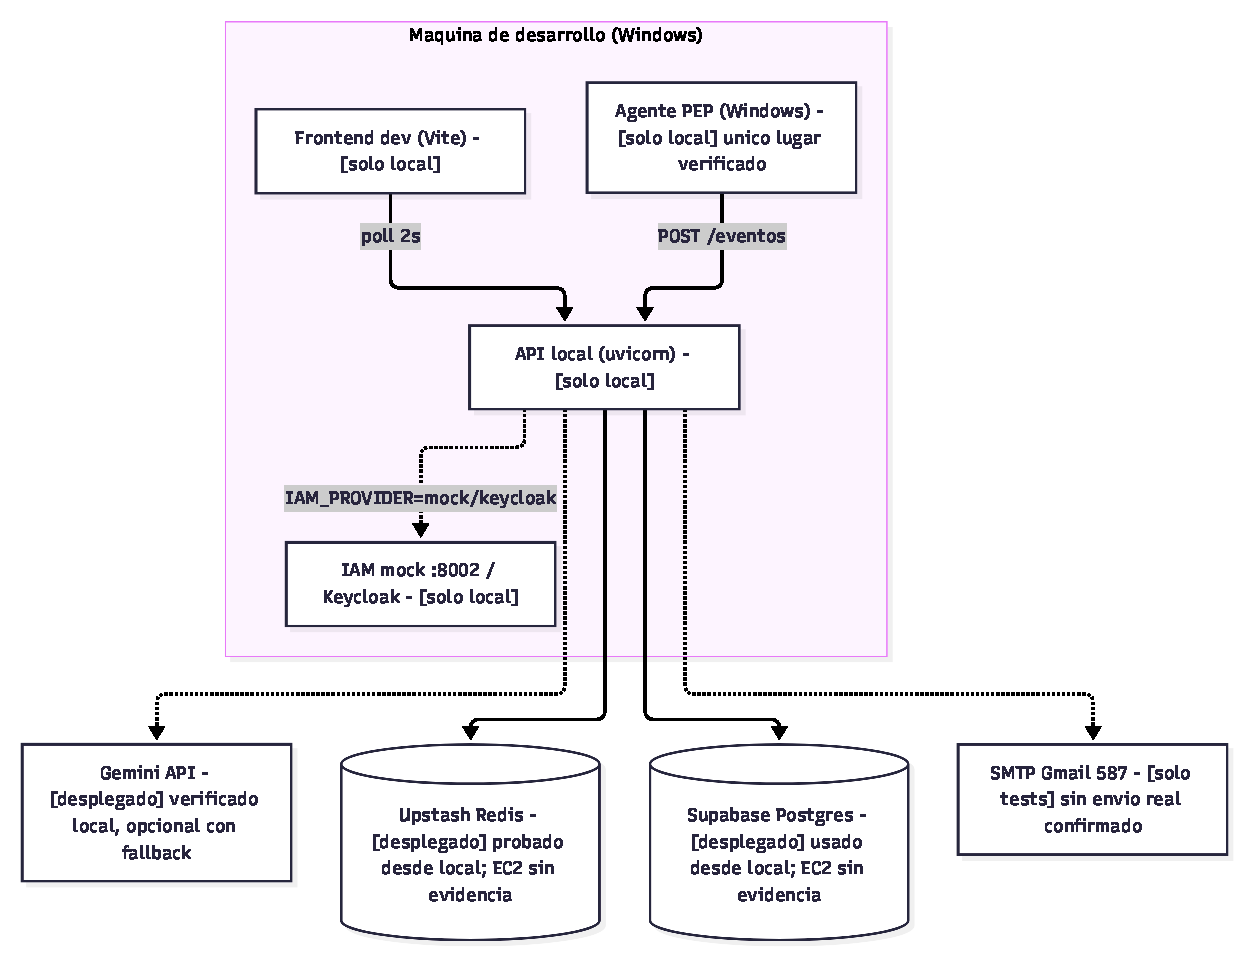
\includegraphics[width=13.5cm]{images/diagramas/v75/despliegue_local.pdf}
	\caption{Arquitectura de despliegue local}
	\label{fig:despliegue-local}
\end{figure}

\subsection{Despliegue en la nube}
La arquitectura de la nube, descripta con Terraform, publica el \emph{dashboard} desde un \emph{bucket} privado a través de una red de distribución de contenidos con HTTPS, que además encamina las solicitudes a la API hacia una instancia de cómputo (figura~\ref{fig:despliegue-aws}). Incorpora las siguientes decisiones de seguridad:
\begin{itemize}
	\item La instancia solo acepta tráfico proveniente de la red de distribución.
	\item El acceso a los metadatos de la instancia exige la versión 2 del servicio, y el disco está cifrado.
	\item Los secretos se guardan en el almacén de parámetros y no en el código.
	\item Las versiones se publican mediante el almacenamiento de objetos y comandos remotos, sin acceso SSH.
	\item La API se ejecuta en modo de autenticación estricta y sin la documentación interactiva expuesta.
\end{itemize}

\begin{figure}[ht]
	\centering
	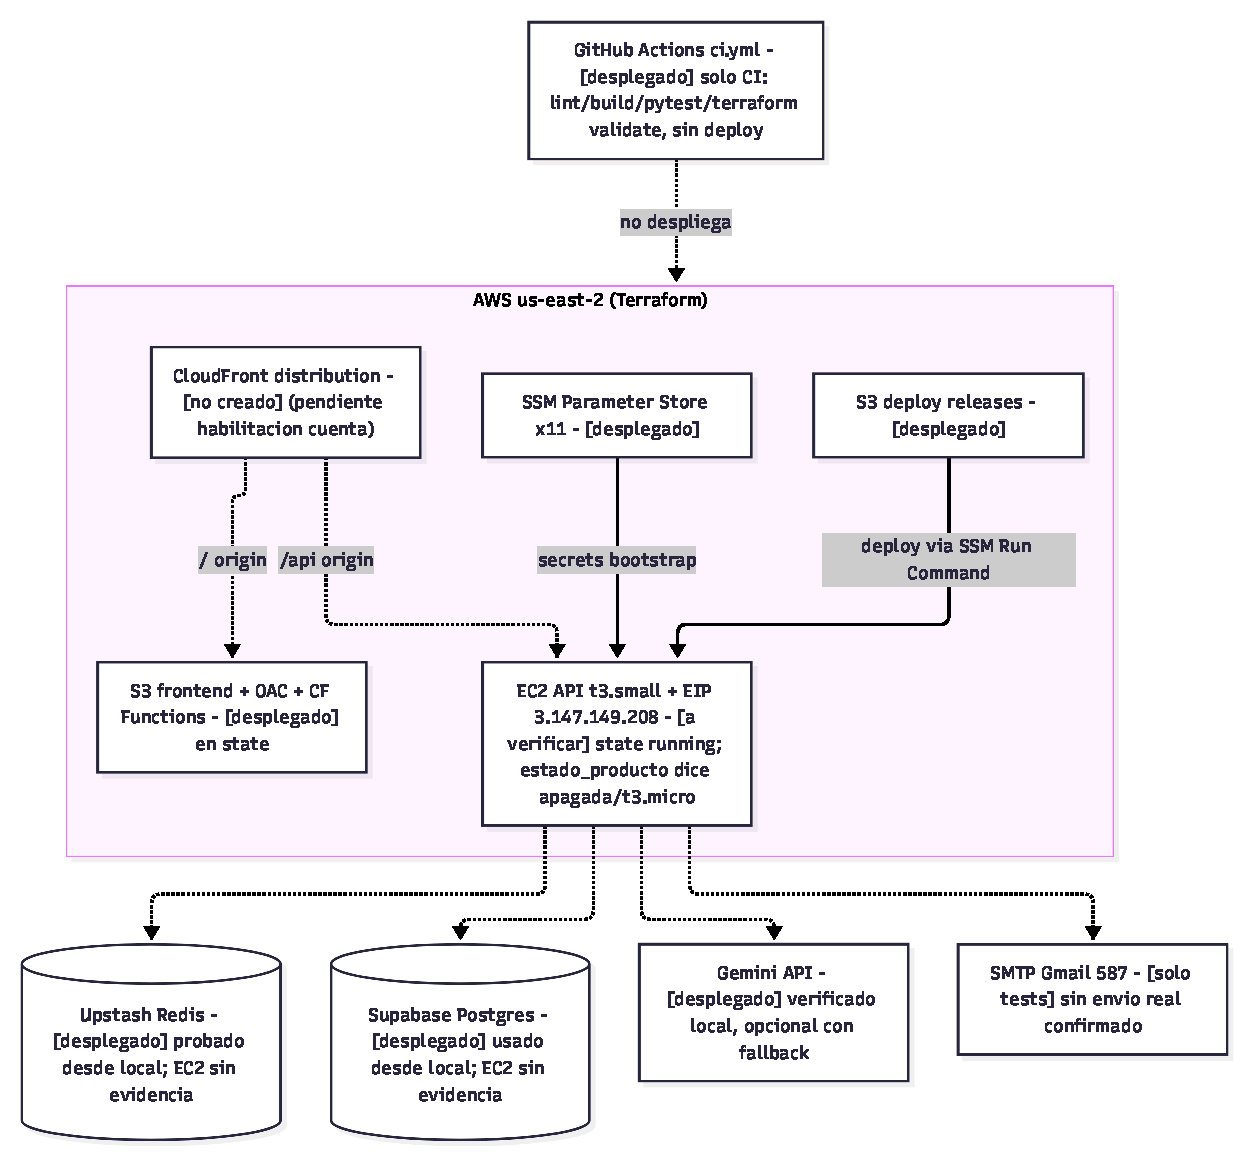
\includegraphics[width=13.5cm]{images/diagramas/v75/despliegue_aws.pdf}
	\caption{Arquitectura de despliegue en la nube, con el estado de cada recurso}
	\label{fig:despliegue-aws}
\end{figure}

La tabla~\ref{tab:diseno-vs-despliegue} contrasta lo diseñado con lo desplegado.

\begin{longtable}{>{\raggedright\arraybackslash}p{4.0cm}>{\raggedright\arraybackslash}p{5.2cm}>{\raggedright\arraybackslash}p{4.9cm}}
	\caption{Arquitectura de la nube: diseño frente a despliegue}
	\label{tab:diseno-vs-despliegue}\\
	\hline
	\textbf{Recurso} & \textbf{Diseño} & \textbf{Estado} \\
	\hline
	\endfirsthead
	\hline
	\textbf{Recurso} & \textbf{Diseño} & \textbf{Estado} \\
	\hline
	\endhead
	Instancia de cómputo de la API & Servidor Linux con la API como servicio del sistema, sin contenedores & Creada; se mantiene apagada fuera de las pruebas para limitar el costo \\
	\hline
	Dirección IP fija, rol de acceso y parámetros de configuración & Identidad de la instancia y secretos administrados & Creados \\
	\hline
	\emph{Buckets} de almacenamiento & \emph{Dashboard} estático y versiones publicadas de la API & Creados \\
	\hline
	Red de distribución de contenidos & HTTPS para el \emph{dashboard} y la API & No creada: la cuenta requiere una habilitación del proveedor \\
	\hline
	Reentrenamiento en la nube & Planificador de la API & Desactivado en la instancia; el reentrenamiento se ejecuta en el entorno local \\
	\hline
	Despliegue continuo & -- & No implementado: la integración continua no despliega \\
	\hline
\end{longtable}

Como la red de distribución no se creó, el despliegue en la nube no tiene un acceso operativo para usuarios finales ni cifrado TLS en ningún tramo. Esta es la causa del estado parcial de RF-02 y del estado no implementado de RNF-13.

\subsection{Contenedores}
Durante el desarrollo se evaluó ejecutar la API, Redis y el \emph{dashboard} con Docker Compose. La alternativa se dejó de lado por tres motivos:
\begin{itemize}
	\item El agente debe ejecutarse de forma nativa en Windows para acceder a los procesos y a los permisos del sistema de archivos, por lo que no podía formar parte de los contenedores.
	\item Redis y PostgreSQL se reemplazaron por servicios gestionados.
	\item Ejecutar la API como servicio nativo en la instancia simplifica la administración con las herramientas del sistema operativo y del proveedor.
\end{itemize}
La imagen de la API se conserva en el repositorio como alternativa de despliegue, pero no forma parte del camino verificado.

\section{Protocolos de comunicación}
\label{sec:protocolos}
\begin{longtable}{>{\raggedright\arraybackslash}p{3.4cm}>{\raggedright\arraybackslash}p{3.2cm}>{\raggedright\arraybackslash}p{7.5cm}}
	\caption{Protocolos de comunicación}
	\label{tab:protocolos}\\
	\hline
	\textbf{Protocolo} & \textbf{Enlace} & \textbf{Justificación} \\
	\hline
	\endfirsthead
	\hline
	\textbf{Protocolo} & \textbf{Enlace} & \textbf{Justificación} \\
	\hline
	\endhead
	HTTP/REST con JSON & Agente $\rightarrow$ API; \emph{dashboard} $\rightarrow$ API & Cada evento es un mensaje discreto con su respuesta, sin necesidad de una conexión persistente. Los contratos están definidos con Pydantic en la API y con Zod en el \emph{dashboard}. \\
	\hline
	Claves en encabezados HTTP & Agente, \emph{dashboard} y administración & Cada agente tiene una clave propia, almacenada como \emph{hash} y revocable. El \emph{dashboard} usa claves separadas para consulta y administración, además del inicio de sesión. Las claves del navegador quedan expuestas al usuario del \emph{dashboard}: un esquema basado en sesiones o \emph{tokens} queda como trabajo futuro. \\
	\hline
	Consulta periódica (2~s) & \emph{Dashboard} $\rightarrow$ API & El puntaje cambia con cada evento, pero ningún caso de uso requiere una notificación instantánea. WebSockets habría agregado manejo de conexión persistente y reconexión sin un beneficio proporcional. \\
	\hline
	RESP con transacciones optimistas & API $\leftrightarrow$ Redis & Actualización atómica del estado del usuario ante eventos concurrentes. \\
	\hline
	Protocolo de PostgreSQL & API $\rightarrow$ PostgreSQL & Protocolo estándar, con grupo de conexiones y tiempos de espera acotados. \\
	\hline
	HTTPS & API $\rightarrow$ Gemini y proveedor IAM; usuario $\rightarrow$ \emph{dashboard} en la nube (diseñado) & Cifrado hacia los servicios externos. En la nube, la red de distribución terminaría TLS para el \emph{dashboard} y para el agente. \\
	\hline
	OAuth 2.0 con credenciales de cliente & API $\rightarrow$ Keycloak & Autenticación de la API ante el proveedor IAM, con el \emph{token} en caché hasta su vencimiento. \\
	\hline
	SMTP con STARTTLS & API $\rightarrow$ servidor de correo & Envío de notificaciones con cifrado del canal. \\
	\hline
	HTTP sin TLS (limitación) & Agente $\rightarrow$ API & En el entorno verificado, el canal no está cifrado y no hay autenticación mutua. Se declara como limitación (RNF-13). \\
	\hline
\end{longtable}

\section{Síntesis}
\label{sec:sintesis-arquitectura}
La arquitectura separa la decisión, centralizada en la API, de la aplicación, distribuida en los agentes, siguiendo el modelo de Zero Trust. Las tecnologías se eligieron por componente: Python para todo lo que toca al modelo, TypeScript para la interfaz y servicios gestionados para el almacenamiento. El sistema está verificado en un despliegue local; el despliegue en la nube está diseñado como código, con controles de seguridad explícitos, y aplicado en forma parcial, sin la capa que provee el cifrado.
